% {
%     \bfseries
%     % \footnotesize
%     \noindent 
%     {
%         \itshape
%         Abstract
%     }.
%     As Dublin City Council asked to study the impact of 
%     COVID-19 on the city-bikes usage as they are planning 
%     to optimize city-bike system. This paper is the 
%     first step that is to investigate the impact of pandemic on the 
%     usage of the city bike network.
%     However, since the limitation of this paper is restricted into 8 papers 
%     and the limited machine tools. 
%     This paper 
%     selected features 
%     (\blue{'station id', 'time', 'bike stands', 'available bike stands', 'available bikes'}) 
%     which is useful for analyzing bike-usage from 
%     the full dataset published by Dublin City Council 
%     \cite{CityBikedataset}.  
%     Moreover, doing more feature engineering to these five features which ultimately 
%     became a time series with one feature of totally 118 bike stations. 
%     By using the regression models introduced in lectures, which are 
%     Ridge and Lasso regression models, this paper 
%     firstly applying $k$-fold cross validation to them on a 
%     sampled dataset. 
%     Considering the Long-Short Term Memory (LSTM) Recurrent Neural Networks (RNNs) 
%     are designed for 
%     handling time series, this paper began with introducing the 
%     concepts of RNNs and the LSTM. 
%     Then applied cross validation to a simple LSTM RNN model, compare
%     with regression models together. 
     

%     \noindent Keywords. Dublin City Bike-usage; Pandemic; Regression Models; Ridge; Lasso; Recurrent Neural Networks (RNNs);
%     Long-Short Term Memory (LSTM)
%     \vspace*{2em}
% }
\chapter{P\normalsize{REPROCESSING}}    
\section{Loading Data Files}
\paragraph{Raw Data}
Row data \cite{CityBikedataset} are included in 41 files, staring from the 2018-10-01 to 
2023-12-25. They included information of Dublin-bikes, in features 
:\blue{ 'station id', 'time', 'last updated', 'name', 'bike stands',
'avaliable bike stands', 'avaliable bikes', 'status', 'address',
'latitude', 'longitude'} for 118 stations in Dublin city. 
% The table below is a demo of row data files

\begin{figure}[H]
    \centering
    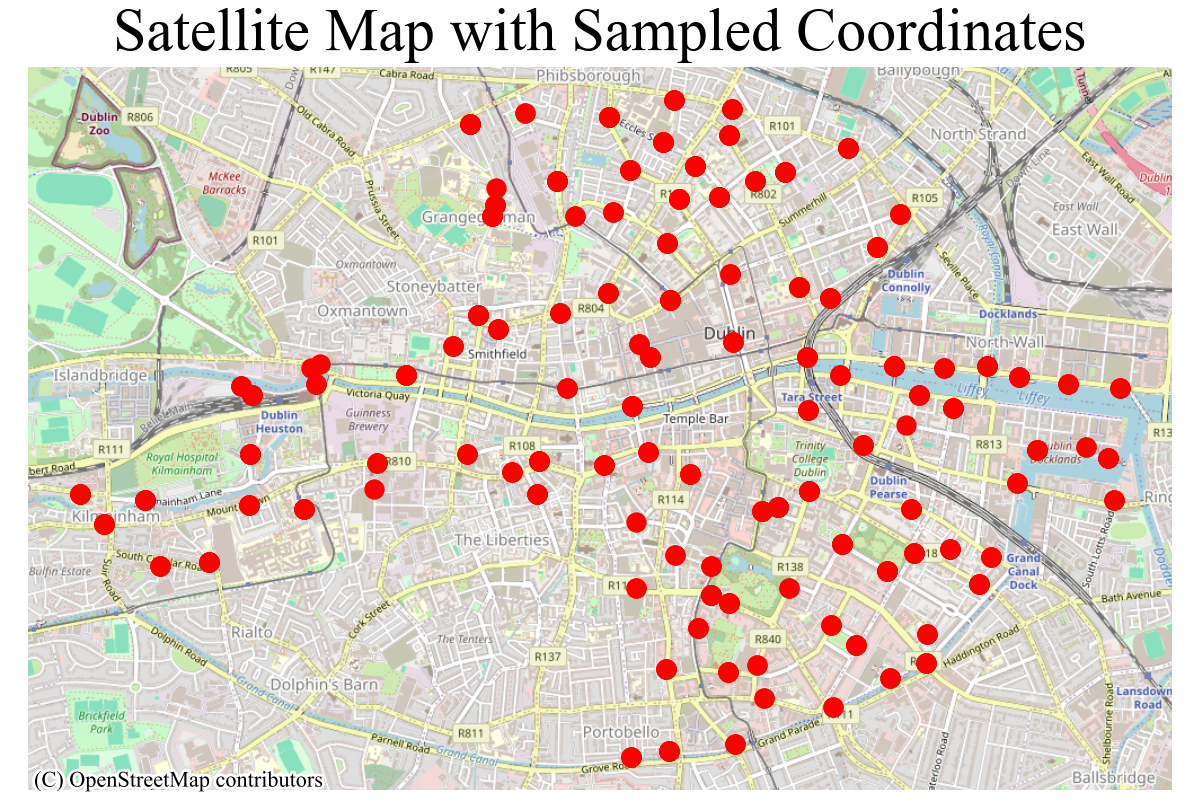
\includegraphics[width=0.45\textwidth]{chap/fig0.png}
    \caption{
        \footnotesize
        Satellite coordinates of bike stations
        } % 表格标题
    \label{FIGURES: CORRD}
\end{figure}

\paragraph{Data Spliting}
In order to handle the tasks, the row data required to be preprocessed before 
staring analysis them. Since the main tasks are assess the impact of the 
pandemic on the city-bike usage, the data files are divided into three parts 
by the time stamps of beginning of city-school were closed 
\cite{OHalloran2020Pandemic} and the 
HSE stopped releasing pandemic figures \cite{OHalloran2022Pandemic}. 
Respectively, the data files 
are stand for before, during and post pandemic periods.

\paragraph{Data Cleaning} 
Besides that, there are two type of features in the files where the one stands for 
city-bike usage and the other one stands for the information of each bike station.
Thus, there will be additional data file for storing the information of all stations 
including \blue{ 'station id', 'name', 'address', 'latitude', 'longitude'}.
Treat the missing values as 0 for all values and delete the repeated sample values.

\paragraph{Rounding}
Considering the pandemic was continued for years and the data were sampling in few 
seconds which is unnecessary for analyzing the general pattern in the large picture 
across years. Thus, excluding load and split raw data files, rounding the 
time stamps to nearest 8 hours and determine the mean of each feature values in 
that 8 hours. Such procedure could reduce the demanding of computation resources and 
make it easier to find general pattern.

\section{Feature Engineering}
\paragraph{Modify Features}
According to the hints, the "bike usage" can be represented by the number of 
bikes have been taken from (or brought to) that station.
The features that can might be use to tasks are 
\blue{'station id', 'time', 'bike stands', 'available bike stands', 'available bikes'}.

Moreover, for a station, the number of available bike stands and available bikes can 
determine the value of total bike stands which is the sumption of them. 
However, available bike stands $(N_{stands}(t))$ and bikes $(N_{bikes}(t))$ 
at some time stamps $(t)$ do not show the usage of bikes. 

In order to solving this problem without 
applying complicate methods, 
define the difference of $N_{stands}(t)$ 
and $N_{bikes}(t)$ as $N_{\text{bring stand bikes}}(t) $ and 
$N_{\text{take bikes}}(t) $ where follow
\[
    \begin{cases}
        N_{\text{bring stand bikes}}(t) 
        = 
        N_{\text{stands}}(t-\Delta t) 
        - 
        N_{\text{stands}}(t) \\
        N_{\text{take bikes}}(t) 
        = 
        N_{\text{bikes}}(t-\Delta t) 
        - 
        N_{\text{bikes}}(t)
    \end{cases}
\]
For $N_{\text{bring stand bikes}}(t)$,
it means that 
there are $N_{\text{bring stand bikes}}(t)$ bike stands 
get a returned bike in 
time interval $[t, t+\Delta]$.
The other $N_{\text{bikes}}(t)$ means that there are
$N_{\text{take bikes}}(t)$ bikes are brought in 
time interval $[t, t+\Delta]$.
After that, 
\[
N_{\text{bring stand bikes}}(t)  + N_{\text{take bikes}}(t) 
\]
the number of bike were using by citizens.
Theoretically, the sumption 
$
N_{\text{bring stand bikes}}(t)  + N_{\text{take bikes}}(t) 
$ equals to $0$
as long as no bikes are used.
At the end of processing, $Z$-score normalize the $3$ separated data files
separately, which make shift the mean of data to $0$ and the 
standard deviation to $1$.
It follows 
\[
    Z = \frac{X - \mu}{\sigma}
\]
where the $X$ is original data and $\mu$, $\sigma$ are mean and 
standard deviation of original data.

Overall, the feature: \blue{'using bikes'} in time interval $[t, t+\Delta]$ are 
\[
    N_{\text{using bikes}}(t) = N_{\text{bring stand bikes}}(t)  +  2N_{\text{take bikes}}(t) 
\]
where the $\Delta = 8$ (hour). It means that there are $N_{\text{using bikes}}(t)$
bikes are used for the station between $t$ and $t+8$ (hour). 
The data with $N$ samples can be formulated as  
\[
   \left\{(t_k, y_k)\right\}_{k = 0}^{N}
\]where $t_k$ is the time of $k^{\text{th}}$ the measurement and 
$y_k$ is the $k$ measurement of \blue{using bikes} in $\left[t_k, t_{k+1}\right]$.

\paragraph{Feature Engineering for Times Series}\label{sec:FeatureEngineerforTimeSeries}
Time series features data has many compositions, it includes 
trends, seasonality, and irregular variations in 
stations analysis. 
The prediction model $\widehat{f}_d$ uses $n$ continues samples to predict 
$q$ step ahead every $d$ time stamp which means 
\[
    \widehat{y}_{k+q} = \widehat{f}_d(y_{k-nd}, y_{k-nd+d}, \cdots, y_{k-d})
\] 
Since various $d$ represent predicting using different cycility, thus using
a combination of $\widehat{f}_d$ to
predict on cycility $d_0,d_1, \cdots, d_m$. Collectively, the prediction model follows
% \[
%     \widehat{y}_{k+q} = 
%     \widehat{f}
%     (y_{k-nd_0}, y_{k-nd_0+d_0}, \cdots, y_{k-d_0}, 
%     \cdots,
%     y_{k-nd_s}, y_{k-nd_s+d_s}, \cdots, y_{k-d_s})
% \]
\begin{align*}
    \widehat{y}_{k+q} = 
    \widehat{f}
    (&y_{k-nd_0}, y_{k-nd_0+d_0}, \cdots, y_{k-d_0}, 
    \\ &\cdots,\\
    &y_{k-nd_s}, y_{k-nd_s+d_s}, \cdots, y_{k-d_s})
\end{align*}
where the parameters $q$, $n$ and $d_0,d_1, \cdots, d_s$ are hyperparameters. 
The processed dataset $y$ has shape
\[
    \left(
        N-(n+1)\max_{i = 0}^{s}
        N_i -q
        , 
        ns
        \right)
\]
where $N_i$ is the number of samples in $d_i$ cycility.
More specific features engineering will be discussed with model designs.

\section{Visualization}
In this part, visualize the bike-usage data in pandemic period of the 
station $3$ and $4$. 
The points at positive region in the \ref{FIGURES: FEATURED DATA} 
mean the bike was took in the at the time step. 
On the contrast, negative value mean the bike was returned bike to station, and 
$0$ means no bike-usage at the time step.
\begin{figure}[H]
    \centering
    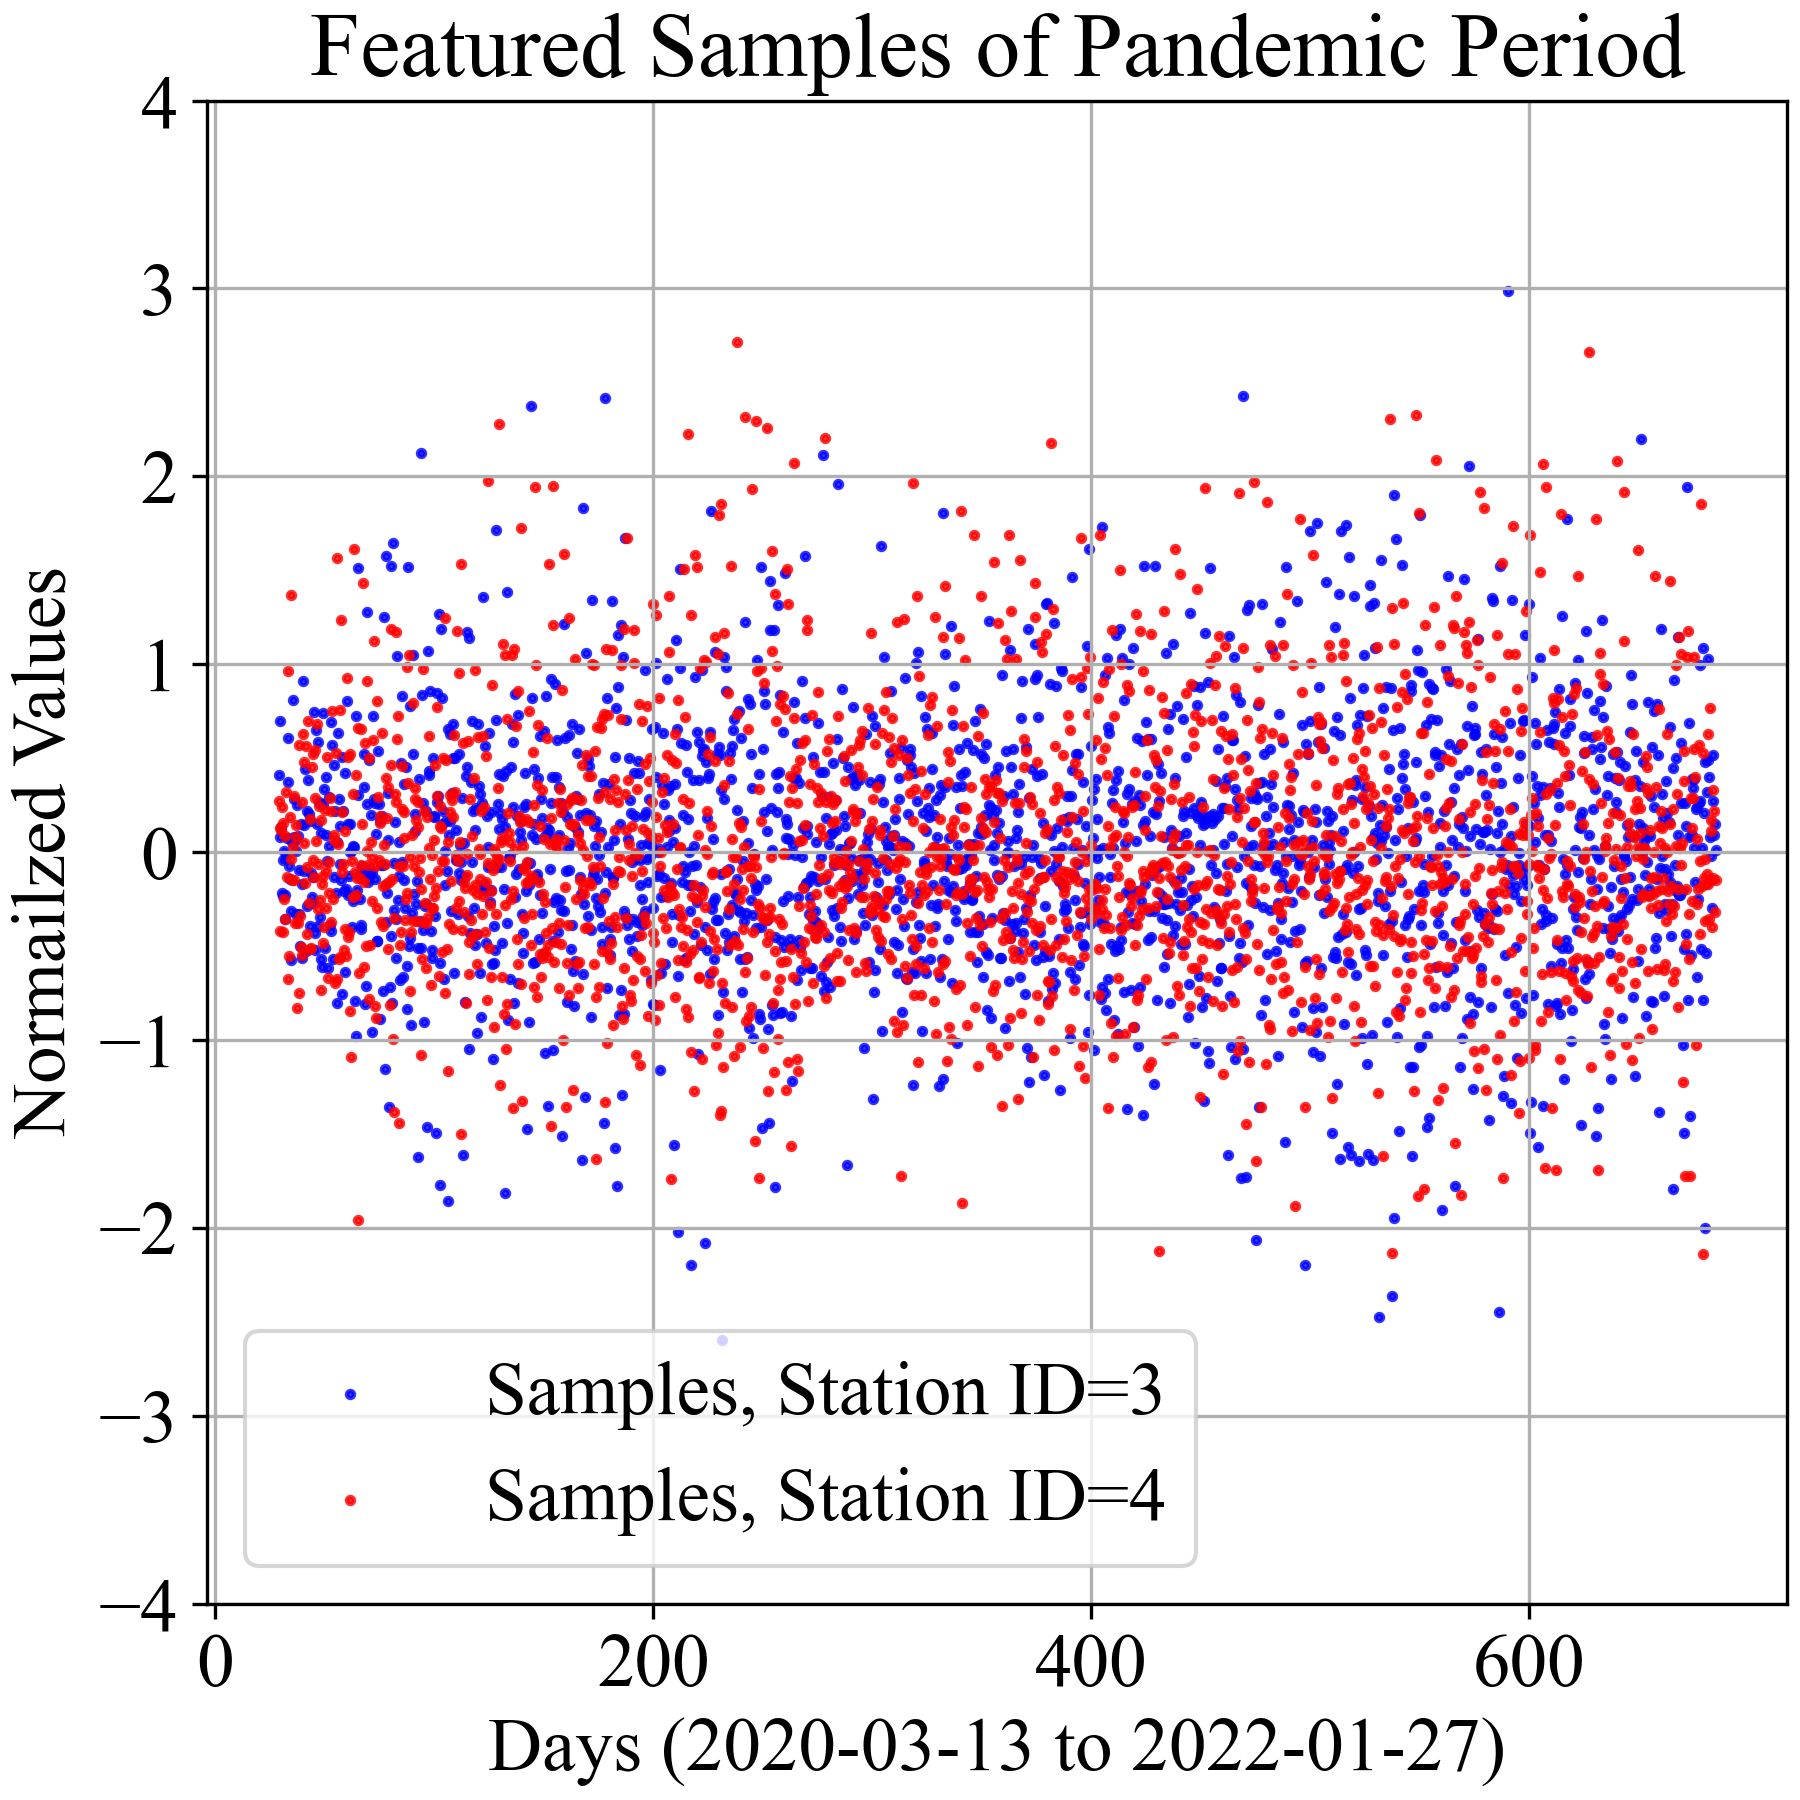
\includegraphics[width=0.35\textwidth]{chap/fig-1.png}
    \caption{
        \footnotesize
        Satellite coordinates of bike stations
        } % 表格标题
    \label{FIGURES: FEATURED DATA}
\end{figure}
% \end{multicols}